% 1999 年全国卷理科第 1 题：集合关系图
% 仅保留 TikZ 矢量源；阴影表示 (M \cap P) \cap \overline S。
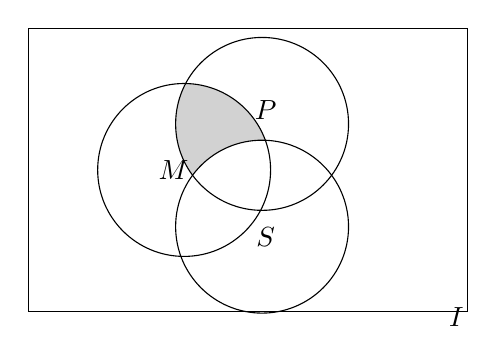
\begin{tikzpicture}[scale=0.9]
  \coordinate (M) at (2.2,2.0);
  \coordinate (P) at (3.3,2.65);
  \coordinate (S) at (3.3,1.2);

  \draw (0,0) rectangle (6.2,4.0);
  \begin{scope}
    \clip (M) circle (1.22);
    \clip (P) circle (1.22);
    \fill[gray!35] (0,0) rectangle (6.2,4.0);
  \end{scope}
  % Erase the part inside S, then redraw all boundaries on top.
  \fill[white] (S) circle (1.22);
  \draw (0,0) rectangle (6.2,4.0);
  \draw (M) circle (1.22);
  \draw (P) circle (1.22);
  \draw (S) circle (1.22);

  \node at (2.05,2.0) {$M$};
  \node at (3.35,2.85) {$P$};
  \node at (3.35,1.05) {$S$};
  \node[below right] at (5.8,0.2) {$I$};
\end{tikzpicture}
